% !TeX root = ../main.tex
\section{Methodology}
\label{sec:methodology}

\begin{figure*}[t]
\centering
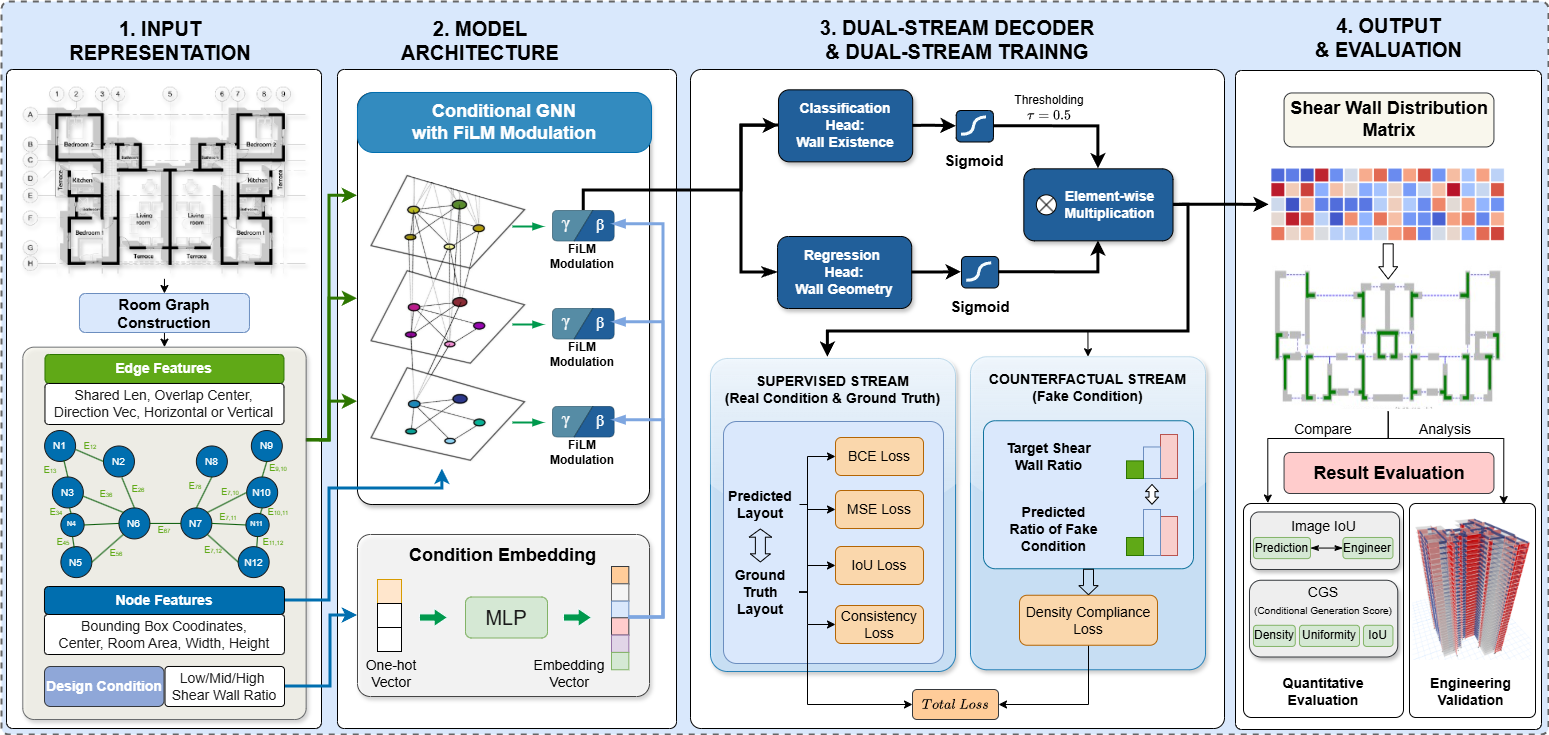
\includegraphics[width=\textwidth]{figs/framework.png}
\caption{The overall framework of the proposed room-level conditional shear wall layout generation method. The pipeline consists of four integrated modules: (1) input representation, transforming architectural plans into room-adjacency graphs with embedded design conditions; (2) model architecture, utilizing a GATv2 backbone with FiLM modulation for feature encoding; (3) dual-stream training, which coordinates supervised learning with counterfactual regularization via a dual-head decoder; and (4) output and evaluation, producing vector-based layouts for engineering validation.}
\label{fig:framework}
\end{figure*}


To address the challenges of semantic alignment and conditional controllability in shear wall design, a unified generative framework is proposed in this study, as illustrated in Fig.~\ref{fig:framework}. The pipeline operates through four integrated stages. First, the \textit{Input Representation} module converts raw CAD plans into room-adjacency graphs, explicitly encoding architectural spaces and design conditions into node and edge features. These graph-structured data are then processed by the \textit{Model Architecture}, which utilizes a GATv2 backbone for spatial feature extraction and a Feature-wise Linear Modulation (FiLM) mechanism for conditional injection.

Subsequently, the framework employs a \textit{Dual-Stream Decoder and Training} strategy, where a decoupled prediction head generates wall existence and geometry. This process is optimized via a hybrid training scheme combining supervised learning on ground-truth data with counterfactual regularization on unmatched conditions. Finally, in the \textit{Output \& Evaluation} stage, the predicted probability matrices are post-processed into vectorized structural layouts for quantitative assessment and engineering validation.

For readability, key symbols used throughout this section are summarized in Table~\ref{tab:notation}.


\begin{table}[t]
\centering
\caption{Notation Summary}
\label{tab:notation}
\small
\begin{tabularx}{\columnwidth}{lX}
\toprule
Symbol & Definition \\
\midrule
$\mathcal{P}$ & Architectural floor plan \\
$G = (\mathcal{V}, \mathcal{E})$ & Room adjacency graph \\
$\mathcal{V} = \{v_1, \ldots, v_N\}$ & Set of $N$ room nodes \\
$\mathcal{E} \subseteq \mathcal{V} \times \mathcal{V}$ & Set of adjacency edges \\
$\mathbf{X} \in \mathbb{R}^{N \times D_v}$ & Node feature matrix ($D_v = 25$) \\
$\mathbf{A} \in \mathbb{R}^{|\mathcal{E}| \times D_e}$ & Edge attribute matrix ($D_e = 8$) \\
$c \in \{0, 1, 2\}$ & Design condition index (low/medium/high) \\
$\mathbf{z}_c \in \mathbb{R}^{D_c}$ & Condition embedding vector ($D_c = 32$) \\
$\mathbf{Y} \in [0,1]^{N \times 16}$ & Ground-truth shear wall layout matrix \\
$\hat{\mathbf{Y}} \in [0,1]^{N \times 16}$ & Predicted shear wall layout matrix \\
$\mathbf{M} \in \{0,1\}^{N \times 16}$ & Constraint mask (1 = wall placement permitted) \\
$\mathcal{N}_i$ & Neighborhood of node $v_i$ \\
\bottomrule
\end{tabularx}
\end{table}

\subsection{Room-based Graph Representation}
\label{subsec:room_graph}

The choice of graph representation is critical for capturing the architectural logic governing shear wall placement. Traditional approaches typically employ a component-level representation, where geometric primitives (e.g., wall segments) serve as edges and their intersections as nodes \cite{zhaoIntelligentDesignShear2023b,zhaoDesignconditioninformedShearWall2023d}. While this preserves detailed topology, it suffers from semantic gaps and computational redundancy.

\begin{figure*}[t]
\centering
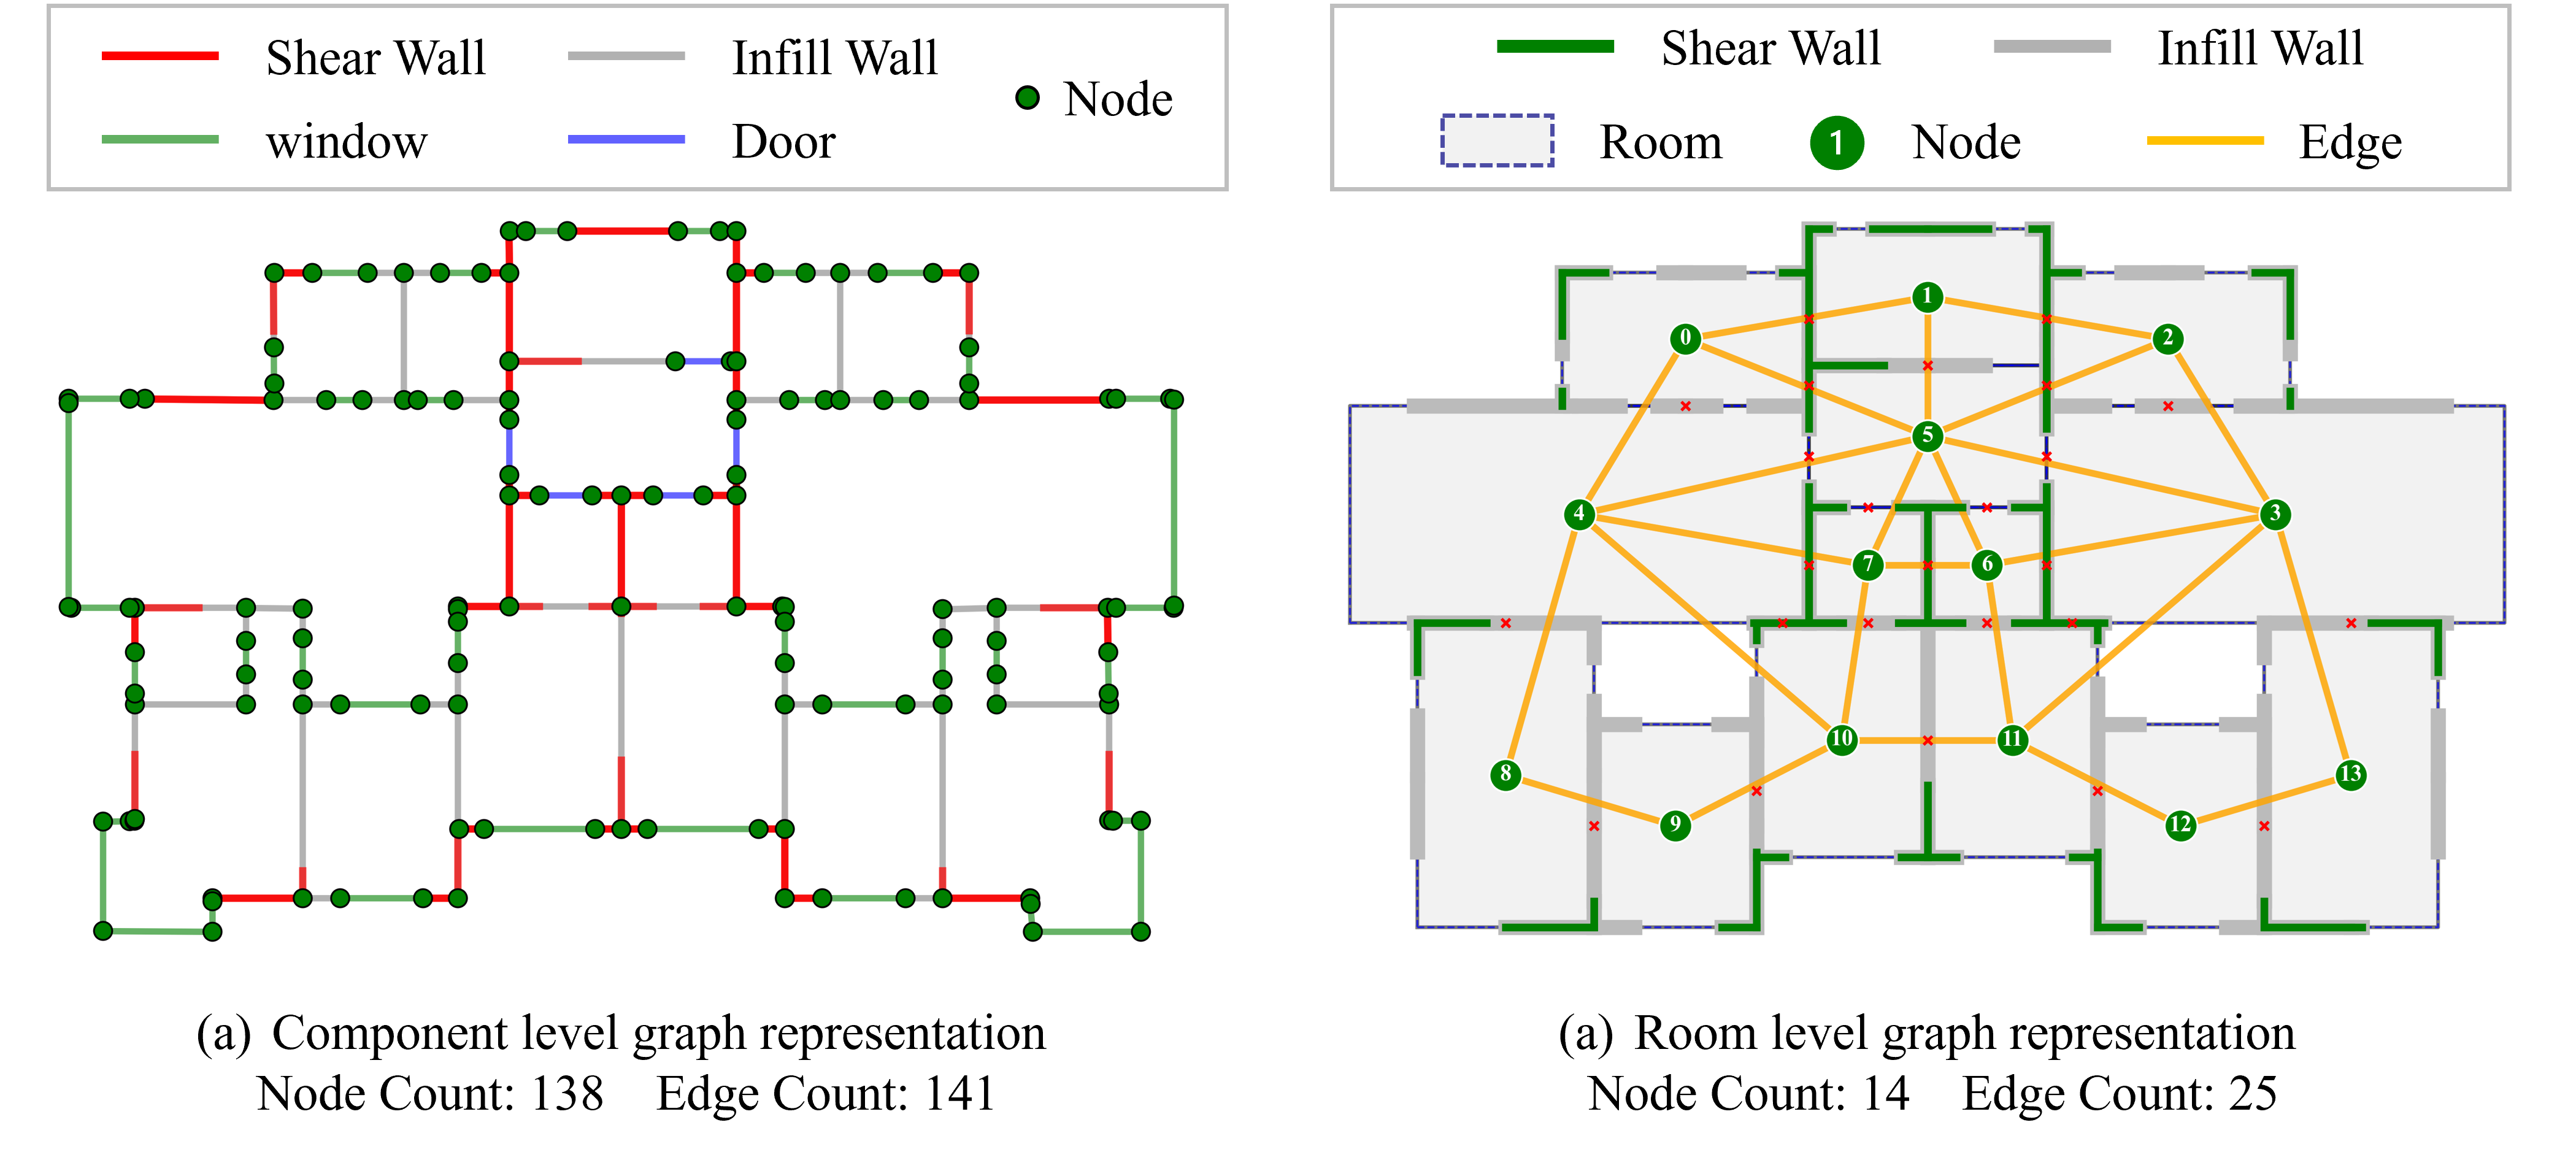
\includegraphics[width=0.8\textwidth]{figs/graph_comparison.png}
\caption{Comparison of graph representations for the same residential floor plan. (a) The component-level representation yields a dense graph (138 nodes, 141 edges) where architectural semantics are fragmented. (b) The proposed room-level representation significantly reduces complexity (14 nodes, 25 edges) while preserving the high-level spatial topology essential for structural layout.}
\label{fig:graph_comparison}
\end{figure*}

As illustrated in Fig.~\ref{fig:graph_comparison}, the limitation of the component-level approach is visually evident: a standard residential plan can generate a graph with over 100 nodes and edges (Fig.~\ref{fig:graph_comparison}a), yet individual wall segments carry little information about the functional spaces they enclose. In contrast, our proposed room-level formulation (Fig.~\ref{fig:graph_comparison}b) elevates the abstraction by modeling functional rooms as nodes and their physical adjacencies as edges.

Modeling floor plans at the room level therefore allows the learning problem to incorporate architectural semantics and boundary feasibility in a compact representation, while remaining compatible with standard message-passing GNNs.
It should be noted that the current formulation assumes rectangular room geometry; non-rectangular spaces are pre-processed via rectilinear decomposition before graph construction (Section~\ref{subsubsec:graph_construction}), and the resulting virtual partition boundaries are excluded from wall placement through the constraint mask. This choice is consistent with prior zoning- and decomposition-based abstractions used to simplify structural design spaces \cite{Claessens_2020,Liu_2021}.


\subsubsection{Graph Construction from Floor Plans}
\label{subsubsec:graph_construction}

Given an architectural floor plan $\mathcal{P}$ in CAD format, the room adjacency graph $G = (\mathcal{V}, \mathcal{E}, \mathbf{X}, \mathbf{A})$ is constructed through the following procedure:

\textbf{Step 1: Room Extraction.} Closed polygonal regions are identified from the CAD drawing through layer-based filtering and contour detection.
Because real-world floor plans frequently contain L-shaped, T-shaped, or otherwise non-rectangular spaces, a rectilinear decomposition algorithm is applied to partition every non-rectangular region into a set of axis-aligned rectangular sub-regions prior to graph construction.
Each resulting rectangular sub-region $r_i$ with area exceeding a minimum threshold is then registered as a room node $v_i$.
Partition boundaries introduced by this decomposition are virtual edges that carry no structural meaning; they are reflected in the constraint mask by setting the corresponding mask entries to zero, so the model cannot predict shear walls along these artificial boundaries.

\textbf{Step 2: Adjacency Detection.} For each pair of rooms $(r_i, r_j)$, the shared boundary length $l_{ij}$ is computed.
An edge $e_{ij}$ is added to $\mathcal{E}$ if $l_{ij}$ exceeds a threshold $\tau_{adj}$ (set to 400mm to exclude minor contacts).

\textbf{Step 3: Feature Extraction.} Node and edge features are computed as described in Sections~\ref{subsubsec:node_features} and~\ref{subsubsec:edge_features}.

\textbf{Step 4: Label Extraction.} For training data, shear wall locations are extracted from structural drawings and mapped to the 16-dimensional output representation (Section~\ref{subsubsec:output_param}).

\subsubsection{Node Feature Design}
\label{subsubsec:node_features}

Each room node $v_i$ is associated with a feature vector $\mathbf{x}_i \in \mathbb{R}^{25}$ comprising geometric descriptors and constraint information.
The normalized geometric feature vector is 9-dimensional, $\mathbf{x}_i^{geo}\in\mathbb{R}^{9}$, defined as
$(x_{min}, y_{min}, x_{max}, y_{max}, w, h, a, x_c, y_c)$, where $(x_{min},y_{min},x_{max},y_{max})$ are the bounding-box coordinates, $w$ and $h$ are the bounding-box width and height, $a$ is the room area, and $(x_c,y_c)$ is the room centroid.
All entries are normalized to $[0,1]$ within a floor plan.
Constraint information is represented by a 16-dimensional buildable mask $\mathbf{m}_i \in \{0,1\}^{16}$ that indicates whether each boundary segment permits shear wall placement.
Specifically, segments occupied by doors, windows, or other openings are marked as non-buildable (value 0), while remaining segments are marked as buildable (value 1).
Table~\ref{tab:node_features} summarizes the full feature specification.

\begin{table}[t]
\centering
\caption{Node Feature Specification}
\label{tab:node_features}
\small
\begin{tabularx}{\columnwidth}{llX}
\toprule
Category & Dimension & Features \\\midrule
Geometric & 4 & Bounding box $(x_{min}, y_{min}, x_{max}, y_{max})$, normalized \\
Geometric & 2 & Bounding-box size $(w, h)$, normalized \\
Geometric & 1 & Area $a$, normalized \\
Geometric & 2 & Centroid coordinates $(x_c, y_c)$, normalized \\
Constraint & 16 & Buildable mask $\mathbf{m}_i \in \{0,1\}^{16}$ \\
\bottomrule
\end{tabularx}
\end{table}

The constraint mask $\mathbf{m}_i$ is aligned with the output parameterization introduced in Section~\ref{subsubsec:output_param}, enabling the model to learn wall placement while explicitly respecting architectural openings.
All geometric features are normalized using min-max scaling computed over the training set to ensure consistent feature magnitudes.

Room function labels (e.g., bedroom, living room, kitchen) would in principle provide additional semantic cues for shear wall placement, as structural engineers routinely consider functional zoning when allocating lateral-load-resisting elements.
However, the open-source dataset employed in this study does not include room-type annotations for individual spaces.
Consequently, functional labels are not incorporated as node features in the current formulation; incorporating them remains a natural direction for future work as annotated datasets become available.

\subsubsection{Edge Feature Design}
\label{subsubsec:edge_features}

Each edge $e_{ij}$ connecting adjacent rooms $v_i$ and $v_j$ is associated with an attribute vector $\mathbf{a}_{ij} \in \mathbb{R}^{8}$.
The edge feature vector is 8-dimensional and consists of the normalized shared boundary length, the normalized overlap centroid $(x_{ov},y_{ov})$ of the shared boundary, a 4-dimensional relative direction indicator (top/bottom/left/right), and a binary orientation flag indicating whether the shared boundary is horizontal.
The complete list of edge attributes is given in Table~\ref{tab:edge_features}.

\begin{table}[t]
\centering
\caption{Edge Feature Specification}
\label{tab:edge_features}
\small
\begin{tabularx}{\columnwidth}{llX}
\toprule
Feature & Dimension & Description \\\midrule
Shared length & 1 & Normalized length of the shared boundary between rooms $i$ and $j$ \\
Overlap centroid & 2 & Normalized centroid coordinates $(x_{ov}, y_{ov})$ of the shared boundary segment \\
Relative direction & 4 & One-hot encoding indicating the relative position (top/bottom/left/right) of the adjacent room \\
Orientation flag & 1 & Binary indicator of boundary orientation (1 = horizontal, 0 = vertical) \\
\bottomrule
\end{tabularx}
\end{table}

The directional encoding enables the model to learn orientation-specific patterns (e.g., walls more common on certain sides of rooms).

\subsubsection{Output Parameterization}
\label{subsubsec:output_param}

The shear wall layout for each room $v_i$ is parameterized as a continuous vector $\mathbf{y}_i \in [0,1]^{16}$.
This parameterization captures wall placement along all four room boundaries with segment-level precision.
An 8-dimensional alternative would regress two coverage ratios for each of the four boundaries (e.g., measured from the two endpoints of each boundary).
However, this representation fails when a wall segment lies in the interior of a boundary without touching either endpoint, as both endpoint-based ratios would be close to zero and the wall could be incorrectly treated as absent.
To avoid this ambiguity, each boundary (top, right, bottom, left) is split at its midpoint into two half-segments, yielding 8 half-segments in total.
Each half-segment is then described by two ratios, which together provide sufficient flexibility to represent walls attached to an endpoint as well as walls located away from endpoints (Fig.~\ref{fig:output_param}).
For each half-segment $k \in \{1, \ldots, 8\}$, two values encode the wall coverage:

$r_k^{start}$: fraction of the half-segment covered by wall starting from the segment's origin

$r_k^{end}$: fraction covered starting from the segment's terminus

The complete output vector is:
\begin{align}
\mathbf{y}_i = [r_1^{start}, r_1^{end}, r_2^{start}, r_2^{end}, \ldots, r_8^{start}, r_8^{end}]
\end{align}
In practice, splitting each boundary into two halves already covers typical engineering layouts, since shear walls are rarely fragmented into many disjoint sub-segments along a single short boundary.
Further subdivision would increase output dimensionality while providing limited additional benefit, and is therefore not adopted in this work.

The resulting 16-dimensional vector $\mathbf{y}_i$ provides a continuous representation capable of encoding various wall configurations. Specifically, values of 1.0 denote full wall coverage, whereas intermediate values represent partial walls. This parameterization flexibly handles cases ranging from complete structural walls to boundaries containing openings, or simply non-structural partitions (represented by zero values), within a unified vector space.

\textbf{Shared-boundary conflict resolution.}
Because adjacent rooms $v_i$ and $v_j$ each independently predict coverage on their shared boundary, their predictions may be mutually inconsistent.
During inference, this is resolved by taking the element-wise maximum of the two predictions for the corresponding boundary entries:
\begin{equation}
\hat{y}_{shared} = \max\!\left(\hat{\mathbf{y}}_i^{(side_j)},\; \hat{\mathbf{y}}_j^{(side_i)}\right),
\label{eq:boundary_union}
\end{equation}
where $side_j$ denotes the boundary slots of room $v_i$ that face room $v_j$, and vice versa.
This union rule is adopted to avoid artificially fragmenting walls: if either room predicts a wall on the shared segment, the wall is retained in the final layout.
The topological consistency loss $\mathcal{L}_{cons}$ (Section~\ref{subsec:training_strategy}) encourages both rooms to reach compatible predictions during training, reducing the frequency and magnitude of such conflicts at inference time.

\begin{figure*}[t]
\centering
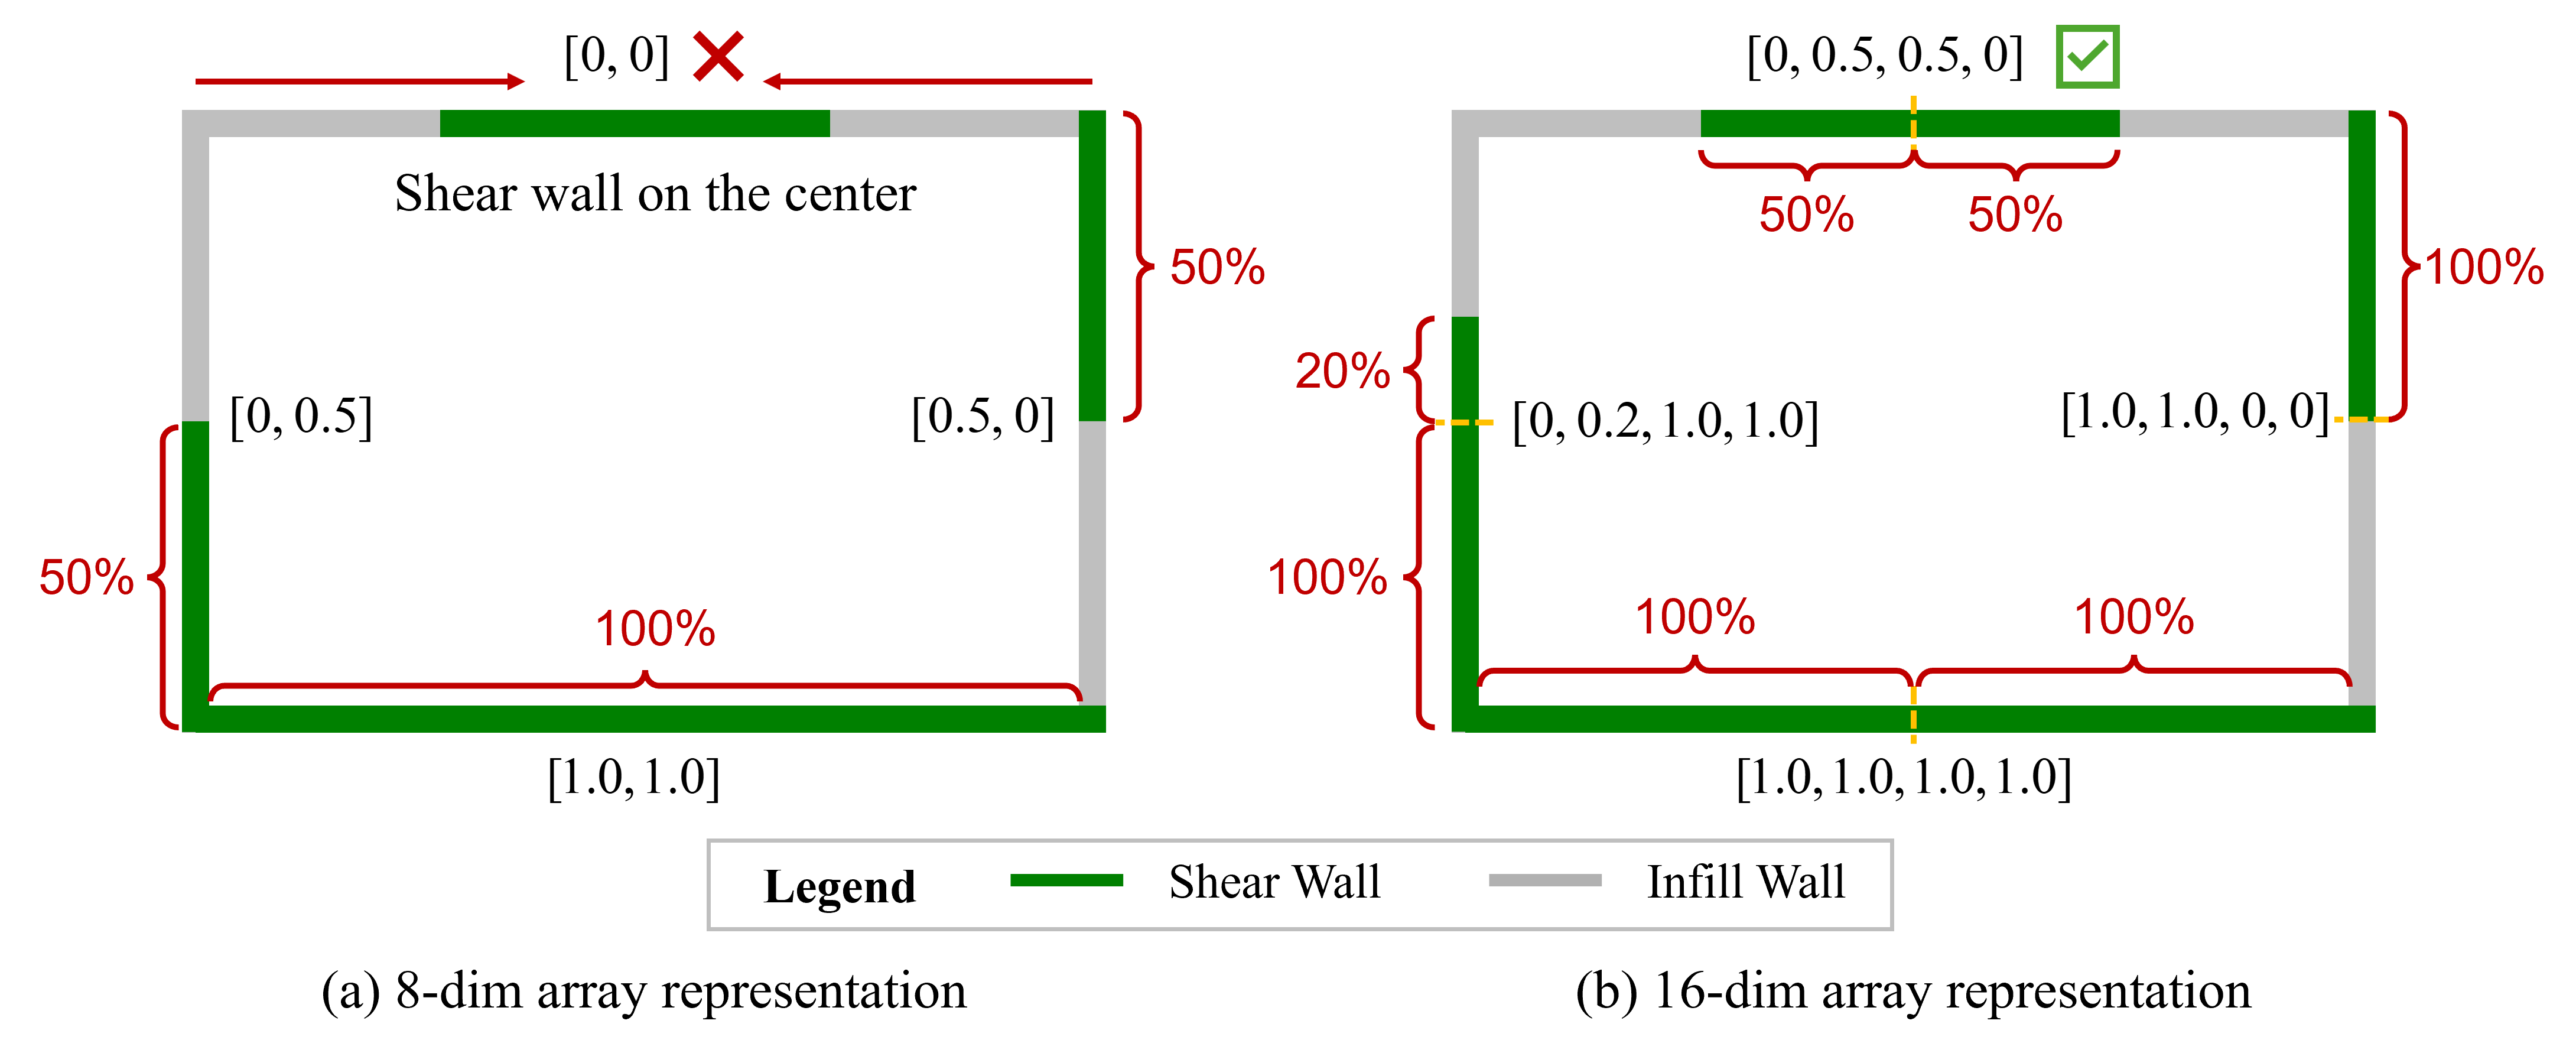
\includegraphics[width=0.85\textwidth]{figs/output_param.png}
\caption{Output parameterization illustration.
A room with four boundaries, each divided into two half-segments.
The 16-dimensional vector maps to wall coverage ratios for each half-segment.}
\label{fig:output_param}
\end{figure*}

\subsection{Problem Formulation}
\label{subsec:problem_formulation}

The shear wall layout generation task is formulated as conditional graph-to-matrix regression.
Given:
\begin{enumerate}
\item Room adjacency graph $G = (\mathcal{V}, \mathcal{E}, \mathbf{X}, \mathbf{A})$ constructed from floor plan $\mathcal{P}$
\item Design condition $c \in \{0, 1, 2\}$ specifying target shear wall density category (low, medium, high)
\item Constraint mask $\mathbf{M} \in \{0,1\}^{N \times 16}$ indicating buildable locations
\end{enumerate}


The objective is to learn a parameterized mapping $f_\theta$:
\begin{equation}
\hat{\mathbf{Y}} = f_\theta(G, c)
\label{eq:method_mapping}
\end{equation}
that predicts the shear wall layout matrix $\hat{\mathbf{Y}} \in [0,1]^{N \times 16}$ approximating the ground-truth layout $\mathbf{Y}$ while respecting physical constraints encoded in $\mathbf{M}$.

The learning objective minimizes a composite loss:
\begin{equation}
\min_\theta \mathbb{E}_{(G, c, \mathbf{Y}) \sim \mathcal{D}} \left[ \mathcal{L}_{sup}(\hat{\mathbf{Y}}, \mathbf{Y}) + \lambda_{phy} \mathcal{L}_{phy}(\hat{\mathbf{Y}}, \mathbf{M}, c) \right]
\label{eq:method_objective}
\end{equation}
where $\mathcal{L}_{sup}$ denotes supervised reconstruction loss and $\mathcal{L}_{phy}$ denotes physics-informed constraints.

Detailed loss formulations are presented in Section~\ref{subsec:training_strategy}.

\subsection{Conditional Graph Neural Network Architecture}
\label{subsec:architecture}

The proposed architecture comprises three components: a GATv2-based encoder for spatial feature aggregation, a FiLM module for conditional injection, and a dual-head decoder for task-decoupled prediction.
Fig.~\ref{fig:network} illustrates the overall architecture.

\begin{figure*}[t]
\centering
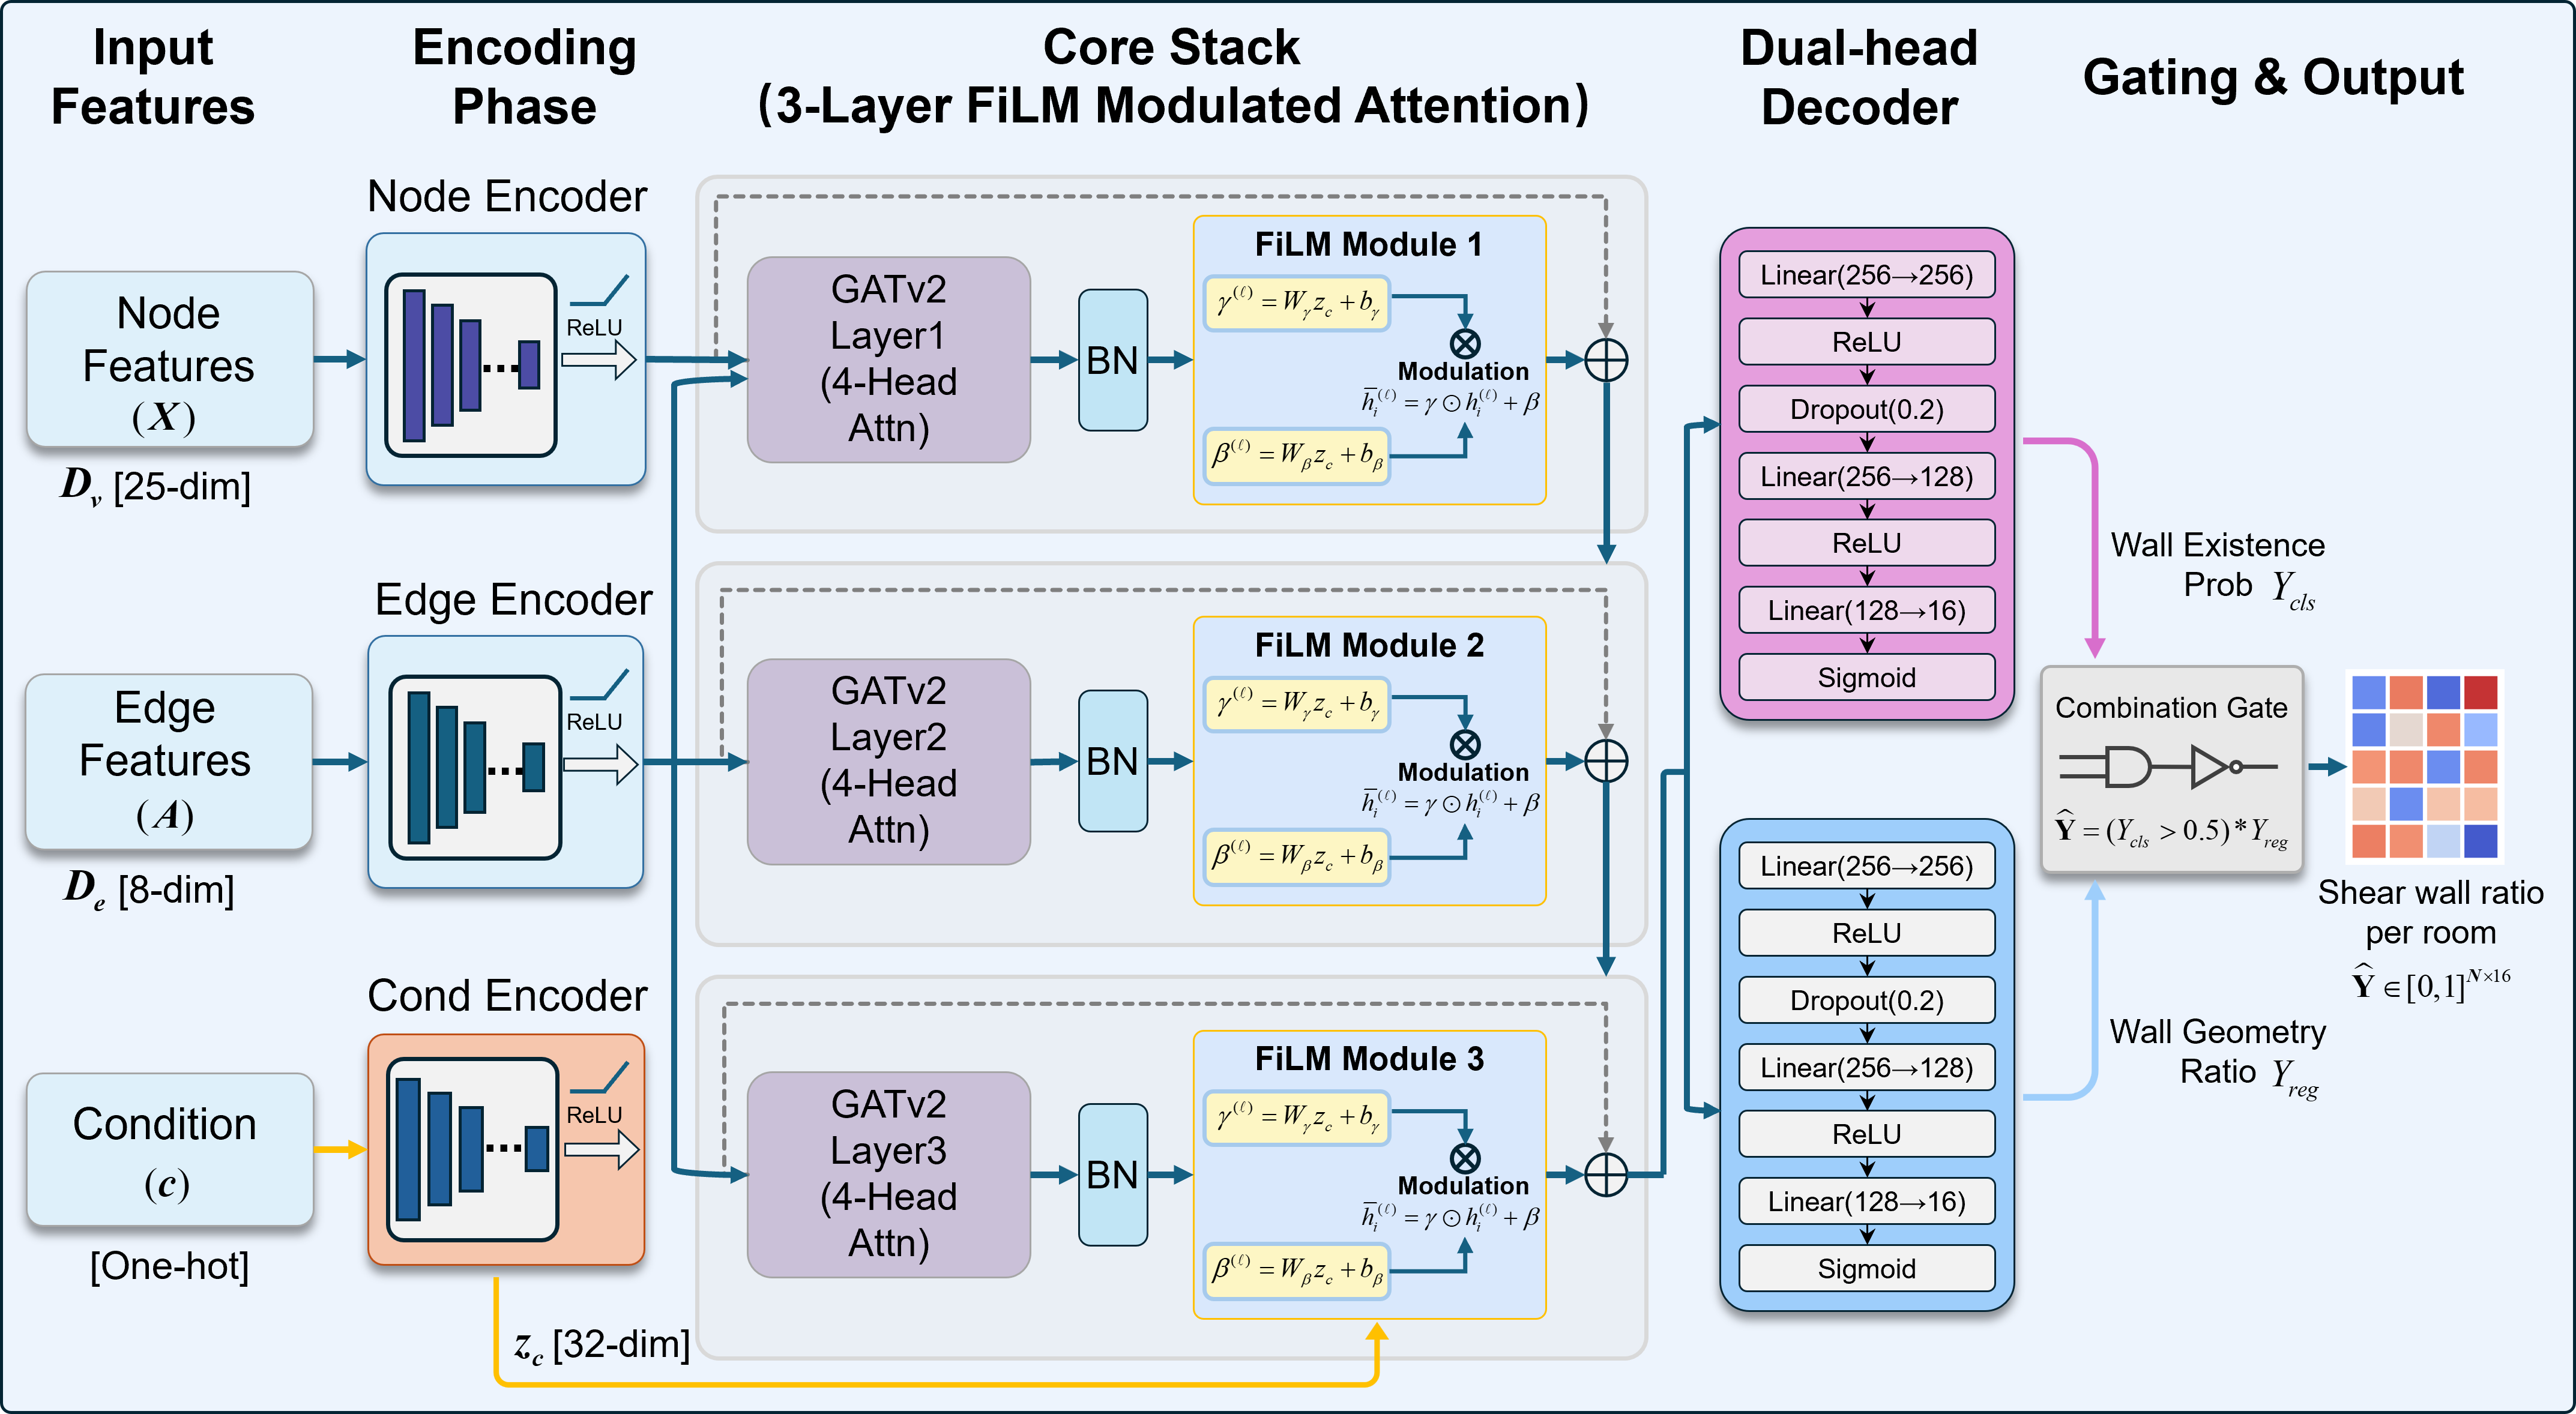
\includegraphics[width=\textwidth]{figs/architecture.png} 
\caption{Model architecture diagram. The architecture consists of: (1) Node and edge encoders, (2) Three GATv2 layers with residual connections, (3) FiLM conditioning applied after each layer, (4) Dual-head decoder producing classification and regression outputs.}
\label{fig:network}
\end{figure*}

\subsubsection{Feature Encoding}

Raw node and edge features are projected to a common hidden dimension $D_h = 256$:
\begin{align}
\mathbf{h}_i^{(0)} &= \text{ReLU}(\mathbf{W}_{node} \mathbf{x}_i + \mathbf{b}_{node}) \\
\mathbf{e}_{ij} &= \text{ReLU}(\mathbf{W}_{edge} \mathbf{a}_{ij} + \mathbf{b}_{edge})
\end{align}
where $\mathbf{W}_{node} \in \mathbb{R}^{D_h \times D_v}$ and $\mathbf{W}_{edge} \in \mathbb{R}^{D_h \times D_e}$ are learnable projection matrices.
The design condition $c$ is embedded through a two-layer MLP:
\begin{equation}
\mathbf{z}_c = \text{MLP}_{cond}(\text{one-hot}(c)) \in \mathbb{R}^{D_c}
\label{eq:method_cond_embed}
\end{equation}
where $D_c = 32$ is the condition embedding dimension.


\subsubsection{GATv2 Backbone for Spatial Aggregation}

Graph Attention Networks v2 (GATv2) serve as the backbone encoder, aggregating information across room neighborhoods through learned attention weights \cite{velickovicGraphAttentionNetworks2018,brodyHowAttentiveAre2022}.
Unlike standard graph convolution variants that use less adaptive neighborhood aggregation, GATv2 dynamically computes attention coefficients based on node pair features, enabling the model to focus on structurally significant neighbors. For node $v_i$ and neighbor $v_j \in \mathcal{N}_i$, the attention coefficient is computed as:
\begin{equation}
e_{ij} = \mathbf{a}^T \text{LeakyReLU}\left(\mathbf{W} [\mathbf{h}_i \| \mathbf{h}_j \| \mathbf{e}_{ij}]\right)
\label{eq:method_gat_attn_logit}
\end{equation}
where $\|$ denotes concatenation, $\mathbf{W}$ is a learnable weight matrix, and $\mathbf{a}$ is a learnable attention vector.

GATv2 differs from standard GAT by applying the nonlinearity after the linear transformation, ensuring strictly dynamic attention computation \cite{brodyHowAttentiveAre2022}. Attention coefficients are normalized via softmax:
\begin{equation}
\alpha_{ij} = \frac{\exp(e_{ij})}{\sum_{k \in \mathcal{N}_i} \exp(e_{ik})}
\label{eq:method_gat_attn_softmax}
\end{equation}

The updated node representation aggregates neighbor features weighted by attention:
\begin{equation}
\mathbf{h}_i' = \sigma\left(\sum_{j \in \mathcal{N}_i} \alpha_{ij} \mathbf{W}_v \mathbf{h}_j\right)
\label{eq:method_gat_update}
\end{equation}

Multi-head attention with $K=4$ heads is employed, with outputs averaged rather than concatenated to maintain dimension consistency:
\begin{equation}
\mathbf{h}_i^{multi} = \frac{1}{K}\sum_{k=1}^{K} \mathbf{h}_i^{'(k)}
\label{eq:method_multihead_avg}
\end{equation}

Three GATv2 layers are stacked with residual connections to enable deep feature propagation while preventing gradient degradation:
\begin{equation}
\mathbf{h}_i^{(\ell+1)} = \mathbf{h}_i^{(\ell)} + \text{GATv2}^{(\ell)}(\mathbf{h}_i^{(\ell)}, \{\mathbf{h}_j^{(\ell)}\}_{j \in \mathcal{N}_i})
\label{eq:method_residual_gat}
\end{equation}


Batch normalization is applied after each GATv2 layer to stabilize training.

\subsubsection{FiLM-based Conditional Injection}

A critical requirement is ensuring generated layouts respect the specified design condition (shear wall density category).
Direct concatenation of condition embeddings with input features often leads to the condition signal being overwhelmed by high-dimensional geometric features during deep propagation, a failure mode related to conditional collapse in generative models \cite{lucasUnderstandingPosteriorCollapse2019}. To address this, Feature-wise Linear Modulation (FiLM) is applied after each GATv2 layer \cite{perezFiLMVisualReasoning2018}.
The condition embedding $\mathbf{z}_c$ is transformed into scaling and shifting parameters:
\begin{align}
\gamma^{(\ell)} &= \mathbf{W}_\gamma^{(\ell)} \mathbf{z}_c + \mathbf{b}_\gamma^{(\ell)} \\
\beta^{(\ell)} &= \mathbf{W}_\beta^{(\ell)} \mathbf{z}_c + \mathbf{b}_\beta^{(\ell)}
\end{align}

These parameters modulate the post-attention features:
\begin{equation}
\tilde{\mathbf{h}}_i^{(\ell)} = \gamma^{(\ell)} \odot \mathbf{h}_i^{(\ell)} + \beta^{(\ell)}
\label{eq:method_film}
\end{equation}
where $\odot$ denotes element-wise multiplication.
cation.
Intuitively, $\gamma$ selectively amplifies features relevant to the target density level, while $\beta$ introduces condition-specific bias.
This late-fusion approach---applying conditioning after initial feature extraction rather than at input---ensures the condition signal influences final predictions without being diluted during early processing.

\subsubsection{Dual-Head Decoder}

Shear wall distributions exhibit sparsity: most boundary segments contain no structural walls.
Direct regression on this sparse target leads to models predicting near-zero values to minimize error, a common issue in sparse-output learning and imbalanced prediction tasks \cite{johnsonSurveyDeepLearning2019}. To address this, the prediction task is decoupled into two sub-tasks handled by parallel decoder, following the general rationale of multi-task decomposition for coupled classification and regression problems \cite{crawshawMultitaskLearningDeep2020,ottJointClassificationTrajectory2022}:

\textbf{Classification Head}: Predicts the probability of wall existence at each of the 16 positions:
\begin{equation}
\hat{\mathbf{Y}}_{cls} = \sigma(\text{MLP}_{cls}(\tilde{\mathbf{H}})) \in [0,1]^{N \times 16}
\label{eq:method_cls_head}
\end{equation}
where $\sigma$ denotes the sigmoid function and $\tilde{\mathbf{H}}$ are the FiLM-modulated features from the final GATv2 layer.

\textbf{Regression Head}: Predicts the geometric parameters (wall length ratios) for each position:
\begin{equation}
\hat{\mathbf{Y}}_{reg} = \sigma(\text{MLP}_{reg}(\tilde{\mathbf{H}})) \in [0,1]^{N \times 16}
\label{eq:method_reg_head}
\end{equation}

Both heads employ identical MLP architectures with three linear layers (256$\to$256$\to$128$\to$16), ReLU activations after the first two layers, and dropout (0.2) after the firDuring inference, the final prediction combines both outputs:
\begin{equation}
\hat{\mathbf{Y}} = \mathbb{I}(\hat{\mathbf{Y}}_{cls} > \tau) \odot \hat{\mathbf{Y}}_{reg}
\label{eq:method_infer_comb}
\end{equation}
where $\tau = 0.5$ is the classification threshold and $\mathbb{I}(\cdot)$ is the indicator function.
 function.
This formulation allows the classification head to establish wall topology while the regression head refines geometric details.

\subsection{Dual-Stream Training Strategy}
\label{subsec:training_strategy}

\subsubsection{Motivation: Addressing Paired Data Scarcity}

Standard conditional generation requires paired training data: multiple outputs (layouts) for the same input (floor plan) under different conditions.
In structural design, this requirement is impractical---each building is typically designed once for a specific set of requirements (seismic zone, building height), yielding only one ground-truth layout per floor plan.
Training solely on available pairs risks the model ignoring condition inputs entirely, learning to predict layouts based on geometric features alone.
This posterior collapse manifests as generated layouts that fail to differentiate across conditions---the model produces similar outputs regardless of specified density requirements.

\subsubsection{Dual-Stream Training Framework}

To mitigate the posterior collapse often seen in conditional generation with limited paired data, a dual-stream training framework is proposed in this study. In the primary supervised stream, the model learns geometric fidelity by minimizing reconstruction losses against the ground-truth layout $\mathbf{Y}_{gt}$ under its true condition $c_{real}$. A density regularization term is also applied in this stream to align the predicted wall quantity with the target density of the real condition. Simultaneously, a counterfactual stream is activated after a warmup period to enforce condition sensitivity. By randomly sampling an alternative condition $c_{fake} \sim \text{Uniform}\{0,1,2\} \setminus \{c_{real}\}$, the network is queried with a mismatched condition on the same floor plan, producing a counterfactual layout $\hat{\mathbf{Y}}_{fake}$. Since no ground truth exists for this synthetic pairing, a density compliance loss is applied to penalize deviations from the expected wall quantity associated with $c_{fake}$. This mechanism creates an explicit gradient signal that couples the output distribution to the condition input, discouraging the model from collapsing to condition-invariant predictions. The overall procedure is summarized in Algorithm~\ref{alg:dual_stream}.


\begin{algorithm}[t]
\caption{Dual-Stream Training}
\label{alg:dual_stream}
\begin{algorithmic}[1]
\REQUIRE Dataset $\mathcal{D}$, model $f_\theta$, epochs $T$, warmup $W$
\ENSURE Trained model $f_\theta$
\FOR{epoch $t = 1$ to $T$}
    \FOR{each batch $(G, c_{real}, \mathbf{Y}_{gt}, \mathbf{M})$ in $\mathcal{D}$}
        \STATE // Supervised Stream
        \STATE $\hat{\mathbf{Y}}_{cls}, \hat{\mathbf{Y}}_{reg} \leftarrow f_\theta(G, c_{real})$
        \STATE $\mathcal{L}_{sup} \leftarrow \mathcal{L}_{BCE}(\hat{\mathbf{Y}}_{cls}, \mathbf{Y}_{gt}) + \lambda_1 \cdot \mathcal{L}_{MSE}(\hat{\mathbf{Y}}_{reg}, \mathbf{Y}_{gt})$
        \STATE \qquad\qquad $+ \lambda_2 \cdot \mathcal{L}_{IoU}(\hat{\mathbf{Y}}_{reg}, \mathbf{Y}_{gt}) + \lambda_3 \cdot \mathcal{L}_{cons}(\hat{\mathbf{Y}}_{reg}, \mathcal{E})$
        \STATE $\mathcal{L}_{phy\_real} \leftarrow \mathcal{L}_{density}(\hat{\mathbf{Y}}_{reg}, c_{real}, \mathbf{M})$
        \STATE
        \STATE // Counterfactual Stream (after warmup)
        \IF{$t > W$}
            \STATE $c_{fake} \leftarrow \text{Uniform}\{0,1,2\}$ \hspace{0.5em} // randomly sampled
            \STATE $\hat{\mathbf{Y}}_{fake} \leftarrow f_\theta(G, c_{fake})$
            \STATE $\mathcal{L}_{phy\_fake} \leftarrow \mathcal{L}_{density}(\hat{\mathbf{Y}}_{fake}, c_{fake}, \mathbf{M})$
            \STATE $\lambda_{cf} \leftarrow \min\bigl(0.1,\; 0.01 \times (t - W)\bigr)$
        \ELSE
            \STATE $\mathcal{L}_{phy\_fake} \leftarrow 0$; \quad $\lambda_{cf} \leftarrow 0$
        \ENDIF
        \STATE
        \STATE $\mathcal{L}_{total} \leftarrow \mathcal{L}_{sup} + 0.05 \cdot \mathcal{L}_{phy\_real} + \lambda_{cf} \cdot \mathcal{L}_{phy\_fake}$
        \STATE Update $\theta$ via backpropagation on $\mathcal{L}_{total}$
    \ENDFOR
\ENDFOR
\end{algorithmic}
\end{algorithm}

A warmup period of $W=20$ epochs is imposed so that the model first acquires basic layout patterns through supervised learning before counterfactual gradients are introduced.
After warmup, the counterfactual weight $\lambda_{cf}$ grows linearly at a rate of $0.01$ per epoch, capped at $0.1$, ensuring a smooth transition that prevents training instability.

\subsubsection{Loss Function Components}

The total loss is organized into three groups: (1) supervised reconstruction losses that directly fit the paired engineering layouts, (2) geometric regularization terms that encourage coherent shapes and boundary agreement, and (3) physics-informed constraints that penalize infeasible placements and enforce condition-dependent density behavior.

\textbf{(1) Supervised reconstruction.} Given the ground-truth layout under the real condition, a classification loss is used to learn the existence of walls, while a regression loss is used to fit the continuous wall-length ratios on positive, buildable segments.
Concretely, the binary cross-entropy for the classification head is defined as:
\begin{equation}
\mathcal{L}_{BCE} = -\frac{1}{N \cdot 16}\sum_{i,j}\left[y_{ij}\log(\hat{y}_{ij}^{cls}) + (1-y_{ij})\log(1-\hat{y}_{ij}^{cls})\right],
\label{eq:loss_bce}
\end{equation}
where $y_{ij} = \mathbb{I}(\mathbf{Y}_{gt}[i,j] > 0.01)$ is the binarized ground-truth.
The regression head is optimized by mean squared error:
\begin{equation}
\mathcal{L}_{MSE} = \frac{1}{|S^+|}\sum_{(i,j) \in S^+}(\hat{y}_{ij}^{reg} - y_{ij}^{gt})^2,
\label{eq:loss_mse}
\end{equation}
where $S^+ = \{(i,j) : y_{ij}^{gt} > 0.01 \land \mathbf{M}[i,j] = 1\}$ restricts the loss to positive samples in buildable regions, preventing collapse to zero predictions.

\textbf{(2) Geometric regularization.} In addition to point-wise regression, global overlap and boundary consistency are encouraged so that predicted layouts form coherent wall patterns aligned with room geometry.
First, a vector-level IoU loss is adopted to optimize holistic overlap between predicted and ground-truth parameter vectors, following the broader use of overlap-based losses in structured prediction and segmentation:
\begin{equation}
\mathcal{L}_{IoU} = 1 - \frac{\sum_{i,j}\min(\hat{y}_{ij}^{reg}, y_{ij}^{gt})}{\sum_{i,j}\max(\hat{y}_{ij}^{reg}, y_{ij}^{gt}) + \epsilon}.
\label{eq:loss_iou}
\end{equation}
Here $\epsilon$ denotes a small constant for numerical stability \cite{huangBatchingSoftIoU2020,zhaoRethinkingDiceLoss2020}.
Second, a topological consistency term is introduced to discourage contradictory predictions on shared room boundaries:
\begin{equation}
\mathcal{L}_{cons} = \sum_{(u,v) \in \mathcal{E}} \left\|\hat{\mathbf{y}}_u^{(side_v)} - \hat{\mathbf{y}}_v^{(side_u)}\right\|^2,
\label{eq:loss_cons}
\end{equation}
where $side_v$ indicates the boundary of room $u$ adjacent to room $v$.

\textbf{(3) Physics-informed density constraint.} To encourage that generated layouts respond to the target design condition, a density compliance loss is imposed on both the supervised and counterfactual streams.
The constraint mask $\mathbf{M}$ is first applied to zero out non-buildable positions, and the resulting effective predictions are averaged across all rooms in each graph to obtain a graph-level density estimate.
This estimated density is then compared against the condition-dependent target $\rho(c)$, which is empirically derived from training-set statistics:
\begin{equation}
\mathcal{L}_{density} = \left(\frac{1}{N}\sum_{i=1}^{N}\sum_{j=1}^{16} \hat{y}_{ij}^{reg} \cdot m_{ij} - \rho(c)\right)^2,
\label{eq:loss_density}
\end{equation}
where $m_{ij}$ is the $(i,j)$-th entry of $\mathbf{M}$, and $\rho(c) \in \{1.57, 3.81, 8.71\}$ are the target average wall quantities for the low, medium, and high density conditions, respectively.

\textbf{(4) Loss weights.} The complete training objective with empirically tuned weights is:
\begin{multline}
\mathcal{L}_{total} = \mathcal{L}_{BCE} + 2.0 \cdot \mathcal{L}_{MSE} + 2.0 \cdot \mathcal{L}_{IoU} \\
+ 0.5 \cdot \mathcal{L}_{cons} + 0.05 \cdot \mathcal{L}_{density}^{real} + \lambda_{cf} \cdot \mathcal{L}_{density}^{fake}
\end{multline}
where $\mathcal{L}_{density}^{real}$ and $\mathcal{L}_{density}^{fake}$ denote the density compliance losses for the supervised and counterfactual streams respectively, with the counterfactual weight $\lambda_{cf}$ following the schedule defined in Algorithm~\ref{alg:dual_stream}.
